\begin{frame}[allowframebreaks]{Data Augmentation}
\begin{itemize}
    \item Data is the fundamental building block of any machine learning algorithm
    \item In several applications we don't have access to unlimited data
    \item So we use Data Augmentation techniques to improve the preformance of our models
    \item Note: It is better to spend time on data rather than fine-scale architecture search in deep learning
\end{itemize}
\framebreak
\begin{itemize}
    \item Create virtual training samples
    \begin{itemize}
        \item Horizontal flip
        \item Random crop
        \item Color casting
        \item Geometric distortion
        \item Translation
        \item Rotation
    \end{itemize}
\end{itemize}
\framebreak
    \begin{figure}
    \centering
    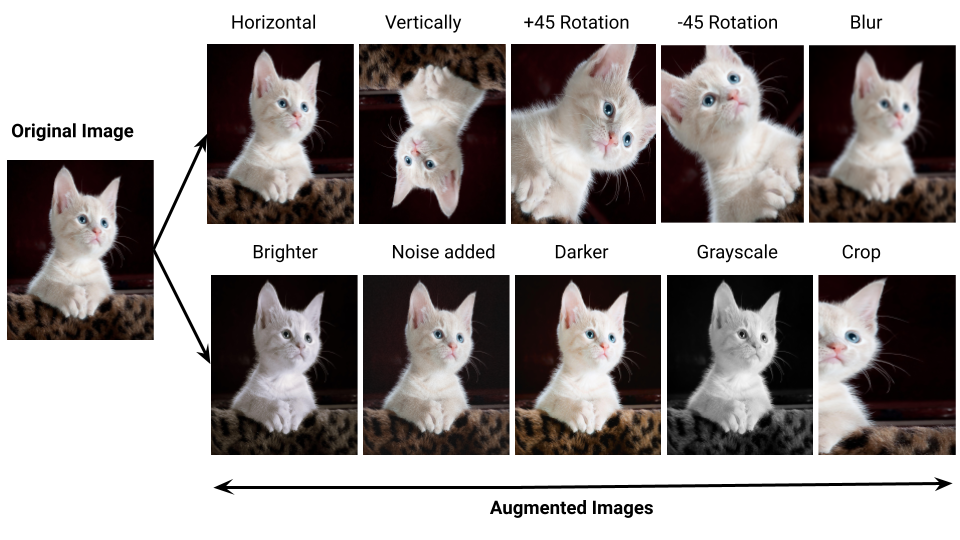
\includegraphics[width=1.0\textwidth,height=1.0\textheight,keepaspectratio]{images/data_augmentation.png}
    \end{figure}
\footnotetext{ \url{https://pranjal-ostwal.medium.com/data-augmentation-for-computer-vision-b88b818b6010}}
\framebreak
\begin{figure}
    \centering
    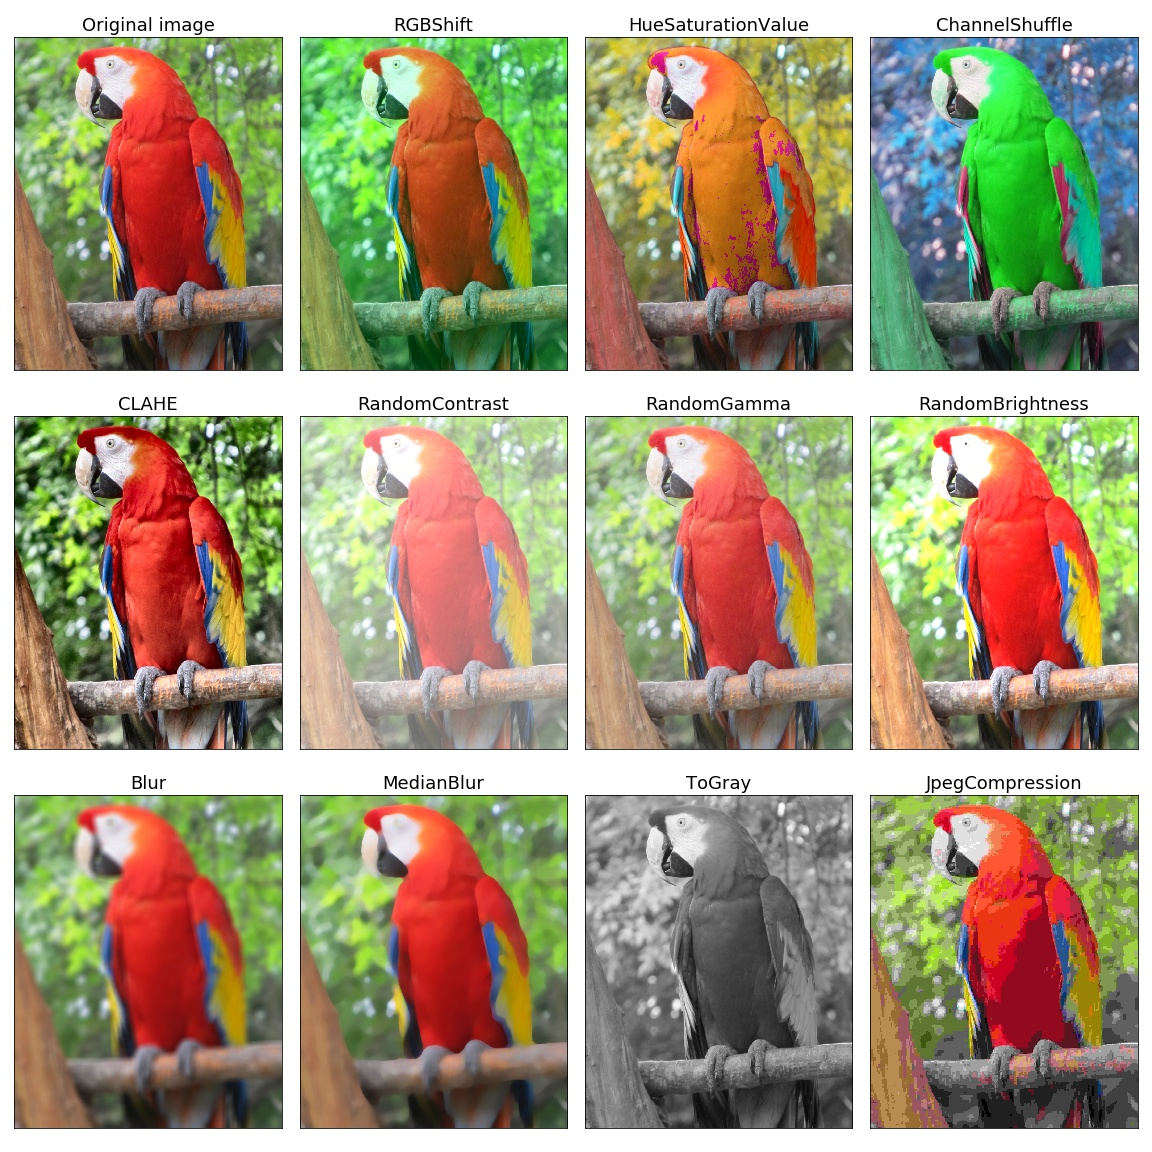
\includegraphics[width=.8\textwidth,height=.8\textheight,keepaspectratio]{images/augmentation_new.jpg}
    \end{figure}
\footnotetext{To simplify data augmentation, tools like  \url{https://github.com/albumentations-team/albumentations}}
\end{frame}

\begin{frame}{Data Augmentation (cont.)}
\begin{itemize}
    \item But, there are many types of augmentations. How do we choose the right ones for our task?
\end{itemize}
\end{frame}

\begin{frame}{Data Augmentation (cont.)}
\begin{itemize}
    \item But, there are many types of augmentations. How do we choose the right ones for our task
    \item \textbf{Answer: Error Analysis} – Identify model weaknesses and apply augmentations that address those issues.
\end{itemize}
\end{frame}

\begin{frame}{Error Analysis for Data Augmentation}
\begin{itemize}
    \item \textbf{Steps:}
    \begin{enumerate}
        \item Train a baseline model.
        \item Make predictions on validation data.
        \item Inspect the worst predictions to identify model weaknesses.
        \item Apply relevant augmentations to address these issues.
    \end{enumerate}
    \item \textbf{Examples:}
    \begin{itemize}
        \item \textbf{Failure with small objects} → Use \textit{Scale Augmentation}.
        \item \textbf{Failure with different colors/environments} → Use \textit{Color Augmentations}.
        \item \textbf{Failure with rotated images} → Use \textit{Rotation Augmentations}.
        \item \textbf{Failure with blurry images} → Use \textit{Noise Augmentations}.
        \item \dots etc.
    \end{itemize}
\end{itemize}
\end{frame}

\begin{frame}{Data Augmentation}
\begin{itemize}
    \item \textbf{Note}: Data augmentation is applied only to the training data.
    \item Applying it to validation/test data \textbf{directly} would lead to \textbf{incorrect evaluation and misleading performance metrics}.
\end{itemize}
\end{frame}

\begin{frame}{Data Augmentation}
\begin{itemize}
       \item However, there is a special inference technique called \textbf{Test-Time Augmentation (TTA)} where multiple augmented versions of the same image are passed through the model separately, and the predictions are averaged to improve accuracy.
\end{itemize}
\begin{figure}
    \centering
    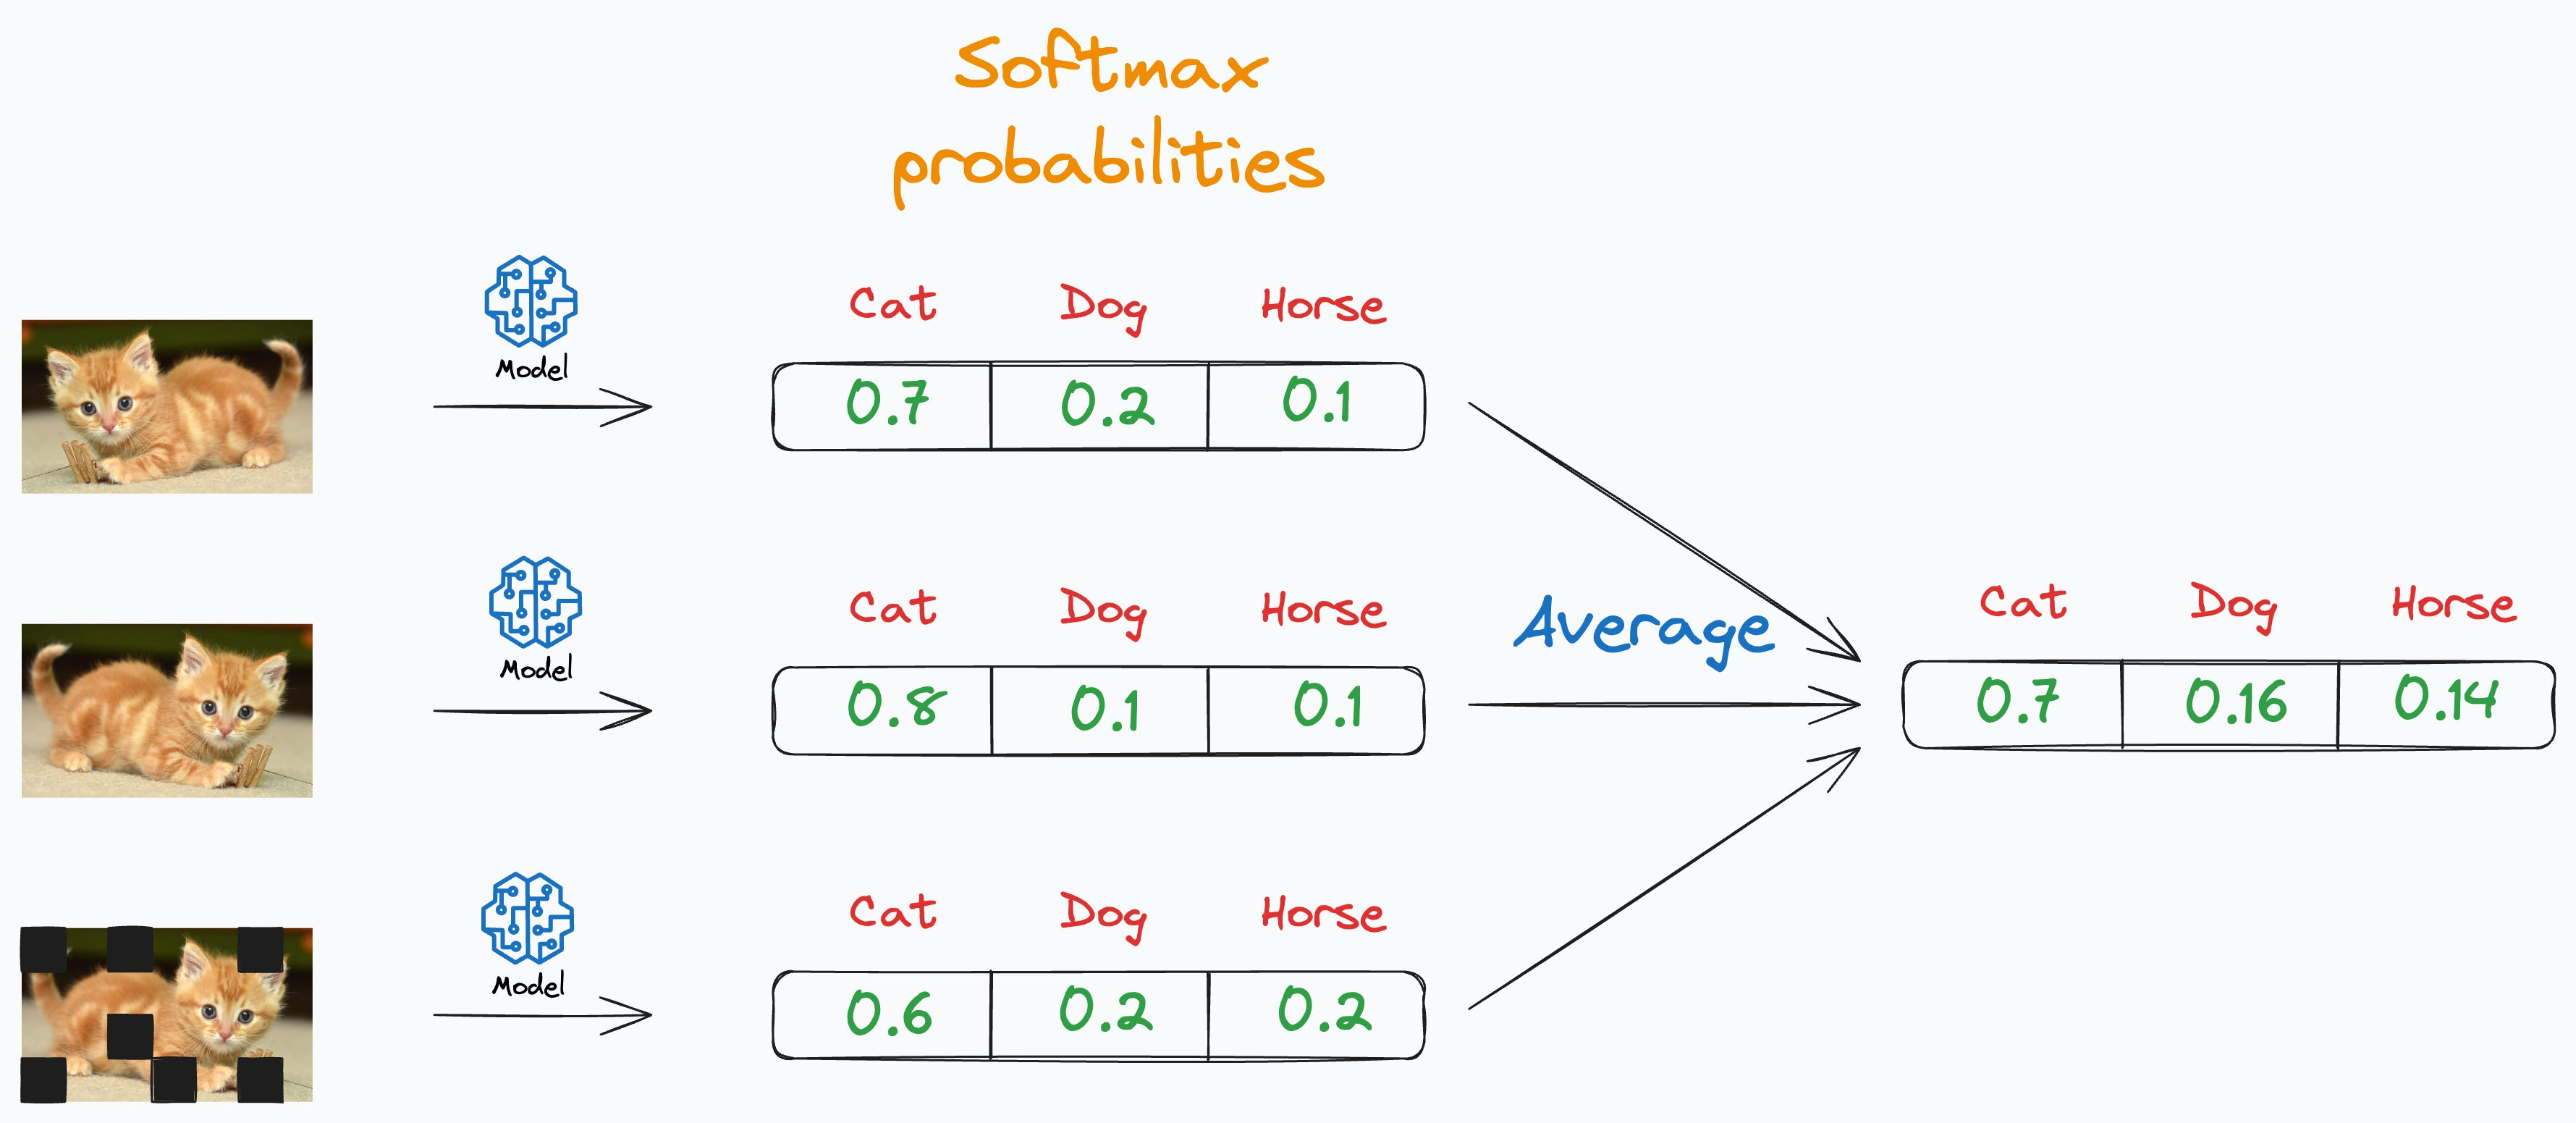
\includegraphics[width=1.0\textwidth,height=1.0\textheight,keepaspectratio]{images/tta.jpg}
    \caption{Test-time Augmentation}
    \end{figure}
\end{frame}

\begin{frame}{Data Augmentation}
\begin{itemize}
    \item TTA is an advanced technique.
    \item Applying it requires \textbf{custom scripts} to generate augmented versions of test images, pass them through the model, and aggregate predictions.
\end{itemize}
\end{frame} 